\section{Análisis de sentimientos}
Para la tarea de análisis de sentimientos se utilizó una base de datos que contiene críticas realizadas por compradores de diferentes tipos de productos de cocina, películas, electrodomésticos y libros. Las reseñas contienen información del usuario que las escribió, ubicación, una calificación para diferentes aspectos como utilidad, ajuste del título, entre otros y finalmente un texto describiendo su opinión de la compra. Las reseñas están separadas en dos clases, positivas y negativas, y por lo tanto dos archivos. Adicionalmente hay un tercer archivo que contiene reseñas para hacer pruebas. A pesar de que el archivo se llama "sin etiqueta" vienen etiquetadas.

\subsection{Procesamiento de la base de datos}

Para el procesamiento de datos se utilizan los archivos llamados \textit{procesados}, por instrucción del profesor. En estos archivos cada línea de texto contiene únicamente las palabras encontradas en las reseñas y su frecuencia asociada, correspondiente a la cantidad de veces que aparecen en esa reseña y al final su etiqueta correspondiente: \textit{positive} o \textit{negative}.\\

Con esto en mente se recorren los archivos buscando generar un diccionario recopilando el todas las palabras que aparecen y almacenando un diccionario por cada reseña con la palabra y las repeticiones que tiene. Esto genero un diccionario de gran tamaño (>190.000 en el caso de la categoría 'libros'), razón por la cual se decidió verificar cuántas palabras tenían frecuencia unitaria una vez construido el \textit{dataset} de cada categoría. Esto mostró que más de 75\% del diccionario correspondía a palabras que aparecían únicamente en una reseña. Con base en esto se procedió a remover estas palabras resultando en un diccionario de menor tamaño. Cabe resaltar que para este vocabulario se utilizaron únicamente palabras del los archivos positivo y negativo, mas no del "sin etiquetas".\\

Con base en el diccionario obtenido para cada categoría se crean dos matrices de tamaño \textit{mxn} donde m corresponde al número de documentos y n al número de palabras del diccionario + 1 (correspondiente a la etiqueta asociada). En la primera matriz se almacena para cada documento la cantidad de veces que contiene cada palabra, constituyendo así el modelo BOW de cada documento. En la segunda matriz se almacena únicamente el hecho de que tenga o no la palabra, generando el modelo BOW booleano. De igual manera, se realiza el proceso para los archivos sin etiqueta obteniendo así seis matrices que se almacenan haciendo uso de la función \url{np.save()} de \textit{NumPy}.\\

En el caso de la unión de todas las categorías se realiza la unión de todos los diccionarios manteniendo únicamente una repetición de cada palabra. Esto genera una diccionario de 100.000 palabras, con base en el cual se realiza el mismo procedimiento previamente mencionado. Se obtienen entonces otras seis matrices de mayor tamaño conteniendo toda la base de datos completa.\\

Ahora bien, para el proceso de extracción de características con base en lexicones se realizo una investigación de cuáles son las características más utilizadas para este tipo de análisis. En \cite{Paper_lexicones} destacan que las principales características que se pueden extraer son \textit{i)} número de palabras positivas \textit{ii)} número de palabras negativas \textit{iii)} palabras positivas divido entre palabras negativas \textit{iv)} polaridad de la última palabra \textit{v)} suma de puntaje de palabras positivas y \textit{vi)} suma de puntaje de palabras negativas. Con esto en mente, se analiza qué información se puede extraer de cada lexicón ofrecido por el profesor resultando en las siguientes características:

\begin{itemize}
    \item Número de palabras positivas de acuerdo con SentiWordNet.
    \item Número de palabras negativas de acuerdo con SentiWordNet.
    \item Total de palabras positivas entre total de palabras negativas.
    \item Polaridad de la última palabra.
    \item Suma de puntajes de palabras negativas.
    \item Suma de puntajes de palabras positivas.
    \item Número de palabras negativas de acuerdo con ANFII.
    \item Número de palabras positivas de acuerdo con ANFII.
    \item Puntaje de palabras negativas.
    \item Puntaje de palabras positivas.
    \item Número de palabras positivas de acuerdo con WordStat.
    \item Número de palabras negativas de acuerdo con WordStat.
    \item Suma de polaridad de las palabras de acuerdo con Senticnet.
\end{itemize}

Esta extracción resulta entonces en una matriz donde las columnas (catorce) corresponden a las características previamente listadas más la etiqueta y las filas corresponden a documentos de los cuales se extrajo la información. Teniendo en cuenta que las características de lexicones no está ligas al \textit{dataset}, la matriz conjunta de todas las categorías se construye juntando las de cada categoría independientemente.

\subsection{Clasificadores}
Para el entrenamiento y comparación de los clasificadores se crea una función que recibe por parámetro un tipo de clasificador que puede ser Regresión Logística (LR), Naive Bayes (NB), Árbol de decisión (DT) o \textit{Random Forest} (RF), un dataset, que puede ser \textit{books}, \textit{dvd}, \textit{kitchen}, \textit{electronics} y \textit{all} y un modelo, que puede ser \textit{bow}, \textit{bool-bow} o \textit{lexicon}. Se utiliza la función \url{train\_test\_split()} de \textit{sklearn}  para obtener datasets separados para entrenamiento (80\%) y validación (20\%). Con estos parámetros se procede a cargar el archivo correspondiente al dataset y modelo indicado y posteriormente a entrenar el clasificador indicado.\\

Este entrenamiento se realiza utilizando la librería \textit{sklearn} de \textit{Python} con los parámetros predeterminados para cada uno de los clasificadores. Posteriormente, se realiza una predicción sobre los datos de validación y con esta se mide \textit{accuracy}, \textit{precision}, \textit{recall} y \textit{f1-score}, nuevamente utilizando la librería \textit{sklearn}. Todos estos valores se almacenan en un DataFrame de pandas para facilitar su comparación.\\

En caso de recibir como parámetro \textit{dataset == all} se utilizan los archivos que contienen todas las categorías mezcladas. A continuación, se comparan los resultados obtenidos.

\subsubsection{Comparación}
Como se indica en las instrucciones de la tarea, se evalúan las cuatro métricas más comunes para medir el desempeño cada uno de los modelos. El resultado de cada métrica se almacena en un DataFrame mostrado a continuación (\textit{véase tabla} \ref{tag:SAresults}). Allí se muestra para cada entrenamiento el \textit{dataset} que se utilizó, el clasificador seleccionado, el modelo escogido y el valor resultante de todas las métricas aplicadas.

\input{resources/SA-df.txt}

Lo anterior muestra claramente que el desempeño en general de todos los modelos es muy similar. No hay un modelo que sobresalga en todas las métricas. A continuación, se muestran promedios de los resultados agrupando para cada parámetro.

\begin{figure}[H]
    \centering
    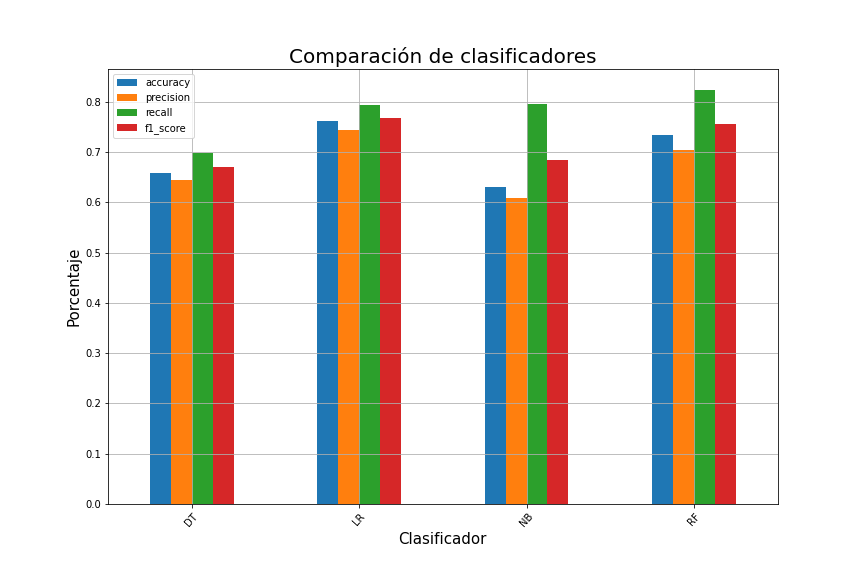
\includegraphics[scale = 0.45]{results/classifier_comparison.png}
    \caption{Comparación de clasificadores}
    \label{fig:classifier_comparisson}
\end{figure}

En la figura \ref{fig:classifier_comparisson} se puede ver el promedio de desempeño de cada uno de los clasificadores probados para cumplir con la tarea de análisis de sentimientos. Se hace evidente que el resultado del árbol de decisión y Naive Bayes son ligeramente inferiores a los demás, con un desempeño promedio de 0.65 y 0.72 respectivamente entre las métricas evaluadas. Esto es ligeramente mejor que adivinar, pues la probabilidad esperada de adivinar correctamente la clase es de 0.50.\\

En contraste los otros dos clasificadores (RF y LR) tienen un desempeño similar, resaltando que el mejor \textit{recall} corresponde a \textit{Random Forest} pero el mejor \textit{precision} corresponde a regresión logística. No obstante, dado que el \textit{recall} de LR es más alto, podría decirse que es el clasificador que mejor clasifica este dataset. 

\begin{figure}[H]
    \centering
    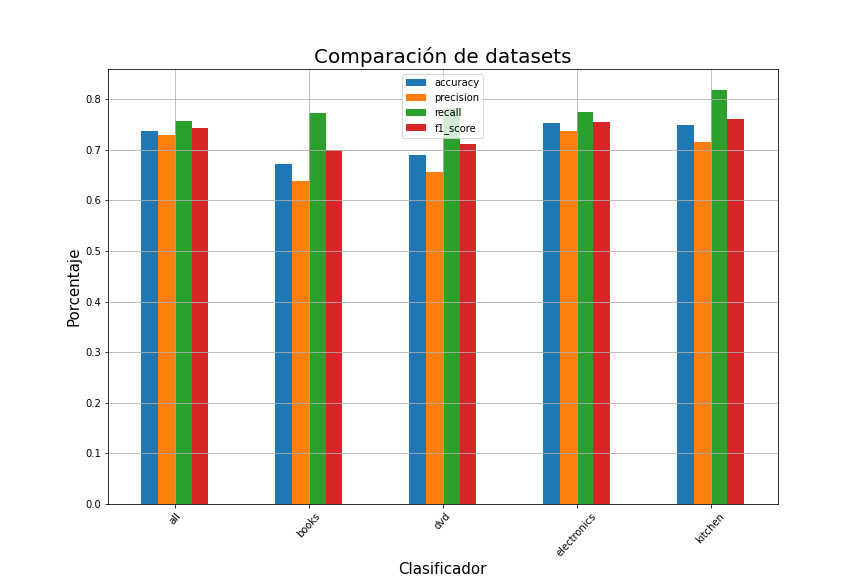
\includegraphics[scale = 0.45]{results/datasets_comparison.png}
    \caption{Comparación de datasets}
    \label{fig:dataset_comparison}
\end{figure}

En cuanto a la comparación de datasets (\textit{véase figura \ref{fig:dataset_comparison}}) los resultados son relativamente similares. En donde hay muy buen \textit{recall} un \textit{precision} bajo compensa. Podría decirse que los datasets de libros y películas son un poco más difíciles de de clasificar, mientas que electrónicos, cocina y todos juntos son un poco más fáciles. Se resalta la poca variación en las métricas resultantes de los clasificadores con todos los \textit{dataset} juntos al igual que en el de electrónicos. Ahora bien, analizando si es preferible o no entrenar modelo para cada categoría o para todas en conjunto, se hace evidente que el rendimiento en general de todos los \textit{datasets} juntos es mejor que los demás. Adicionalmente, solo se requiere un modelo. No obstante, es pertinente resaltar que el tamaño de la matriz de características del dataset 'all' es mayor, pues corresponde a la unión de los diccionarios asociados a cada categoría.

\begin{figure}[H]
    \centering
    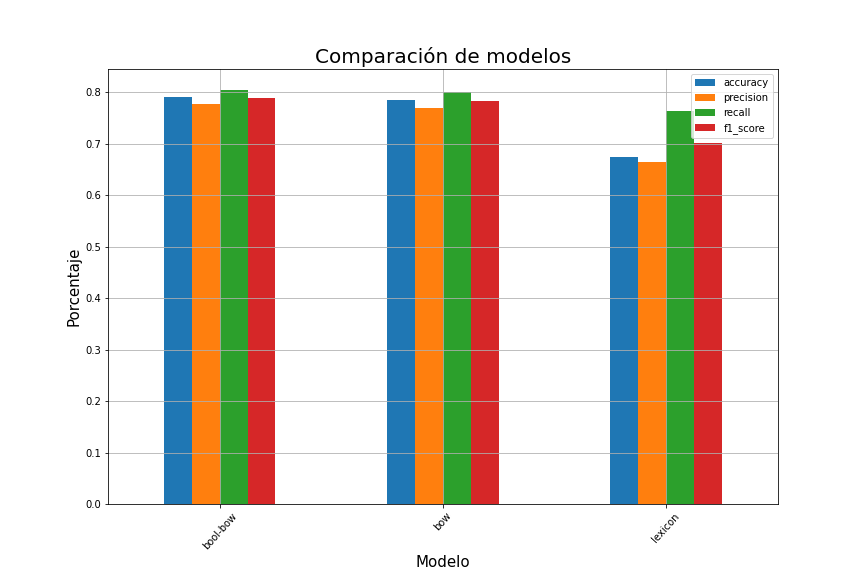
\includegraphics[scale = 0.45]{results/model_comparison.png}
    \caption{Comparación de modelos}
    \label{fig:model_comparisson}
\end{figure}

Ahora bien, los modelos de \textit{Bag of Words} booleano y no booleano tienen resultados casi que idénticos. Los resultados de los modelos de lexicones tienen resultados ligeramente menores, resaltando que \textit{recall} es bastante alto. Adicionalmente, la construcción de cada uno de los modelos no tiene mayor diferencia ni en tiempo ni en capacidad computacional requerida para ejecución o para entrenamiento de los modelos.

\textbf{Característica más importante para regresión logística}\\
Ahora bien, se desea verificar cuál es la característica más importarte para el clasificador de Regresión Logística. Para ello, se obtiene el vector de coeficientes asociado a cada uno de los clasificadores y se busca cuál es el mayor y por consiguiente a qué palabra o característica está asociado. Los resultados se muestran en la tabla \ref{tab:LR-features}.

% Please add the following required packages to your document preamble:
% \usepackage{multirow}
\begin{table}[]
\centering
\caption{Características más importantes para LR}
\label{tab:LR-features}
\begin{tabular}{|l|l|l|}
\hline
\textbf{Categoría}           & \textbf{Modelo} & \textbf{Característica}            \\ \hline
\multirow{3}{*}{Books}       & Bool-BOW        & \multirow{2}{*}{'excellent'}       \\ \cline{2-2}
                             & BOW             &                                    \\ \cline{2-3} 
                             & Lexicon         & \# of negative words  SentiWordNet \\ \hline
\multirow{3}{*}{DVD}         & Bool-BOW        & 'great'                            \\ \cline{2-3} 
                             & BOW             & 'excellent'                        \\ \cline{2-3} 
                             & Lexicon         & \# of negative words  SentiWordNet \\ \hline
\multirow{3}{*}{Electronics} & Bool-BOW        & 'great'                            \\ \cline{2-3} 
                             & BOW             & 'great'                            \\ \cline{2-3} 
                             & Lexicon         & \# of negative words  SentiWordNet \\ \hline
\multirow{3}{*}{Kitchen}     & Bool-BOW        & 'great'                            \\ \cline{2-3} 
                             & BOW             & 'great'                            \\ \cline{2-3} 
                             & Lexicon         & \# of negative words  SentiWordNet \\ \hline
\multirow{3}{*}{All}         & Bool-BOW        & 'excellent'                        \\ \cline{2-3} 
                             & BOW             & 'excellent'                        \\ \cline{2-3} 
                             & Lexicon         & \# of positive words ANFII         \\ \hline
\end{tabular}
\end{table}

\subsubsection{Variación de parámetros de Random Forest}
Se procede a hacer variación de parámetros para el modelo de Random Forest. Se utiliza RandomSearchCV, una función de Sklearn que permite hacer una variación de parámetros aleatoria. En esta función se define cuál es la métrica que se busca maximizar; en este caso se utilizan \textit{precison} y \textit{recall}. Se indica entonces, según recomendación de \cite{Sklearn-RF} que los parámetros a variar son \textit{n\_estimadores} que corresponde al número de estimadores, \textit{max\_features} que corresponde al método para obtener el número máximo de características a tener en cuenta, \textit{criterion} que corresponde al algoritmo a utilizar para el entrenamiento del árbol, \textit{max\_depth} que corresponde a la profundidad máxima del árbol y \textit{max\_leaf\_nodes} que indica el número máximo de nodos 'hojas' (\textit{véase descripción a continuación)}.\\

La variación de los resultados con diferentes parámetros es realmente mínima. Como se puede apreciar en el \textit{notebook} correspondiente. No obstante, los mejores resultados se ven al utilizar log2 como número máximo de características, lo cuál es respaldado por la teoría\cite{Sklearn-RF} en donde afirman que esta es la mejor escogencia para tareas de clasificación.

\subsubsection{Evaluación de los modelos}
Se selecciona entonces el mejor modelo para cada categoría y se evalúa su desempeño en el \textit{dataset} de evaluación. Los resultados se muestran en al tabla \ref{tab:model_eval}
\begin{table}[]
\centering
\caption{Evaluación de modelos}
\label{tab:model_eval}
\begin{tabular}{|l|l|l|l|l|l|}
\hline
\textbf{Categoría} & \textbf{Modelo}     & \textbf{Accuracy} & \textbf{Precision} & \textbf{Recall} & \textbf{F1-score} \\ \hline
Books              & Logistic regression & 0.828             & 0.825              & 0.838           & 0.832             \\ \hline
Kitchen            & Logistic regression & 0.874             & 0.875              & 0.871           & 0.873             \\ \hline
DVD                & Random Forest       & 0.808             & 0.781              & 0.861           & 0.819             \\ \hline
Electronics        & Logistic Regression & 0.863             & 0.861              & 0.869           & 0.865             \\ \hline
All                & Random Forest       & 0.843             & 0.858              & 0.823           & 0.840             \\ \hline
\end{tabular}
\end{table}

\subsection{\textit{Decision tree and random forests}}

A continuación, se realiza un investigación detallada en los modelos de clasificación de árbol de decisión y \textit{Random forest}. Para ello se responden las siguientes preguntas:
\begin{itemize}
    \item \textbf{¿Qué es un árbol de decisión y cómo funciona?}\\
    
    Los árboles de decisión corresponden a un método supervisado de clasificación y/o regresión de \textit{Machine Learning}. Usualmente, un árbol está constituido por nodos, ramas y hojas. En los nodos se evalúa el valor de cierto atributo o característica. Las ramas conectan nodos con otros nodos y con hojas. Las hojas son nodos terminales que predicen la clase o la distribución.\\
    Hay dos tipos de árboles de decisión: árboles de clasificación y árboles de regresión. Los primeros involucran datos discretos mientras que los segundos trabajan con datos continuos \cite{Sklearn-DT}. \\
    El funcionamiento se basa en iniciar con un nodo terminal que es en donde se sabrá la clase a la que pertenece la observación. Luego se selecciona un atributo de la observación y se analizan los posibles valores que puede tomar y la incidencia de dicho atributo en la clase seleccionada. Este proceso se sigue recursivamente hasta llegar un criterio de parada. En cada uno de los nodos se selecciona la mejor división según un determinado criterio, los cuales se muestran a continuación:
    \begin{equation}
        gini(v) = 1-\sum_{y \in L} p(y|v)^2
    \end{equation}
    \begin{equation}
        entropy(v) = -\sum_{y \in L} p(y|v) \cdot log(p(p|v))
    \end{equation}
    Para determinar qué tan bien se comporta una condición se compara el grado de impureza del nodo padre con el grado de impureza de los nodos hijos. Entre mayor sea la diferencia mejor resultaría dividir bajo esa condición.  
    
    \item \textbf{¿Cuál algoritmo se utiliza para construir un árbol de decisión?}\\
    
    A continuación se mencionan los principales algoritmos de entrenamiento de árboles de decisión. La información se obtiene de \cite{Sklearn-DT}.
    \begin{itemize}
        \item \textit{Iterative Dichotomiser 3:} El algoritmo crea un árbol con múltiples caminos evaluando para cada nodo cuál es la característica categórica que ofrece la mayor ganancia de información (information gain) para las etiquetas de clase. El árbol crece hacia abajo hasta alcanzar su tamaño máximo y se aplica una etapa de \textit{pruning} o poda. 
        \item \textit{C4.5:} Es el sucesor del algoritmo previamente descrito. Retira la condición de que las características deben ser categóricas definiendo dinámicamente atributos discretos que permiten partir el atributo continuo en diferentes sets de intervalos.
        \item \textit{C5.0:} Es una versión mejorada de C4.5 que utiliza menos memoria y crea sets de decisión más pequeños siendo más acertado. Está liberado bajo licencia de propiedad.
        \item \textit{\textbf{CART:}} Es similar a C4.5 pero soporta objetivos numéricos (regresión). Construye árboles binarios usando la característica que más ganancia de información ofrezca en cada nodo. Es el utilizado por \textit{scikit-learn}.
    \end{itemize}
    \item \textbf{¿Un árbol de decisión es un modelo generativo o discriminativo?}\\
    
    La diferencia fundamental entre un modelo discriminativo y uno generativo radica en que el modelo discriminativo se aprende las diferencias entre clases mientras que el generativo modela la distribución de las clases individuales. Por esto mismo los árboles de decisión son modelos discriminativos. A través de condicionales y reglas de decisión el árbol va decidiendo si una observación específica se encuentra dentro de una clase o de la otra. \cite{DvsG}.
    
    \item \textbf{¿Qué es un método agrupado en \textit{Machine Learning}?}\\
    
    Un método de aprendizaje agrupado o \textit{ensemble learning} hace referencia a cuando agrupan varios modelos base con el fin de obtener una predicción óptima. Resulta preferible confiar en varios modelos que en uno solo. Adicionalmente, utilizar un conjunto de modelos ocasiona que le modelo sea más resistente a \textit{overfitting}.\\
    Es necesario asegurarse de que los modelos utilizados en el conjunto son independientes. Esto puede garantizarse utilizando diferentes tipos de algoritmos (redes neuronales, regresión logística, árboles de decisión, SVMs, etc.) o entrenando un mismo modelo con diferentes datos. Se pueden utilizar diferentes técnicas para garantizar la independecia de estos sets de datos como \textit{bagging}, \textit{boosting}, \textit{stacking}, entre otros.  
    
    \item \textbf{¿Qué es \textit{bagging}?}\\
    
    \textit{Bootstrap aggregating} o \textit{B-agging} es un algoritmo utilizado para mejorar la estabilidad de conjuntos de modelos (\textit{ensembles}) tanto de regresión como de clasificación.\\
    El método consiste en muestrear con reemplazo el dataset original generando una nueva cantidad de sub-datasets que pueden tener observaciones duplicadas pero que de seguro tienen observaciones nuevas. Este método se conoce como \textit{Bootstrap}. La decisión final respeto a la etiqueta de la observación se obtiene usando \textit{Aggregation}. Se puede realizar con base en el total de salidas o en la probabilidad de las predicciones.
    
    \item \textbf{¿Qué es \textit{Random Forest} y cómo funciona?¿\textit{Random Forest} utiliza \textit{bagging}?}\\
    
    De manera general, \textit{Random Forest} corresponde a un conjunto de múltiples árboles de decisión buscando obtener una predicción más acertada y estable, usualmente entrenados utilizando \textit{bagging}. En la figura \ref{fig:RF} se muestra de mejor manera su procedimiento. Como se mencionó previamente es importante que los modelos (en este caso los árboles) sean independientes y tengan correlación muy baja. Es en este punto donde interviene el método de \textit{bagging}.\\
    
    \begin{figure}[H]
        \centering
        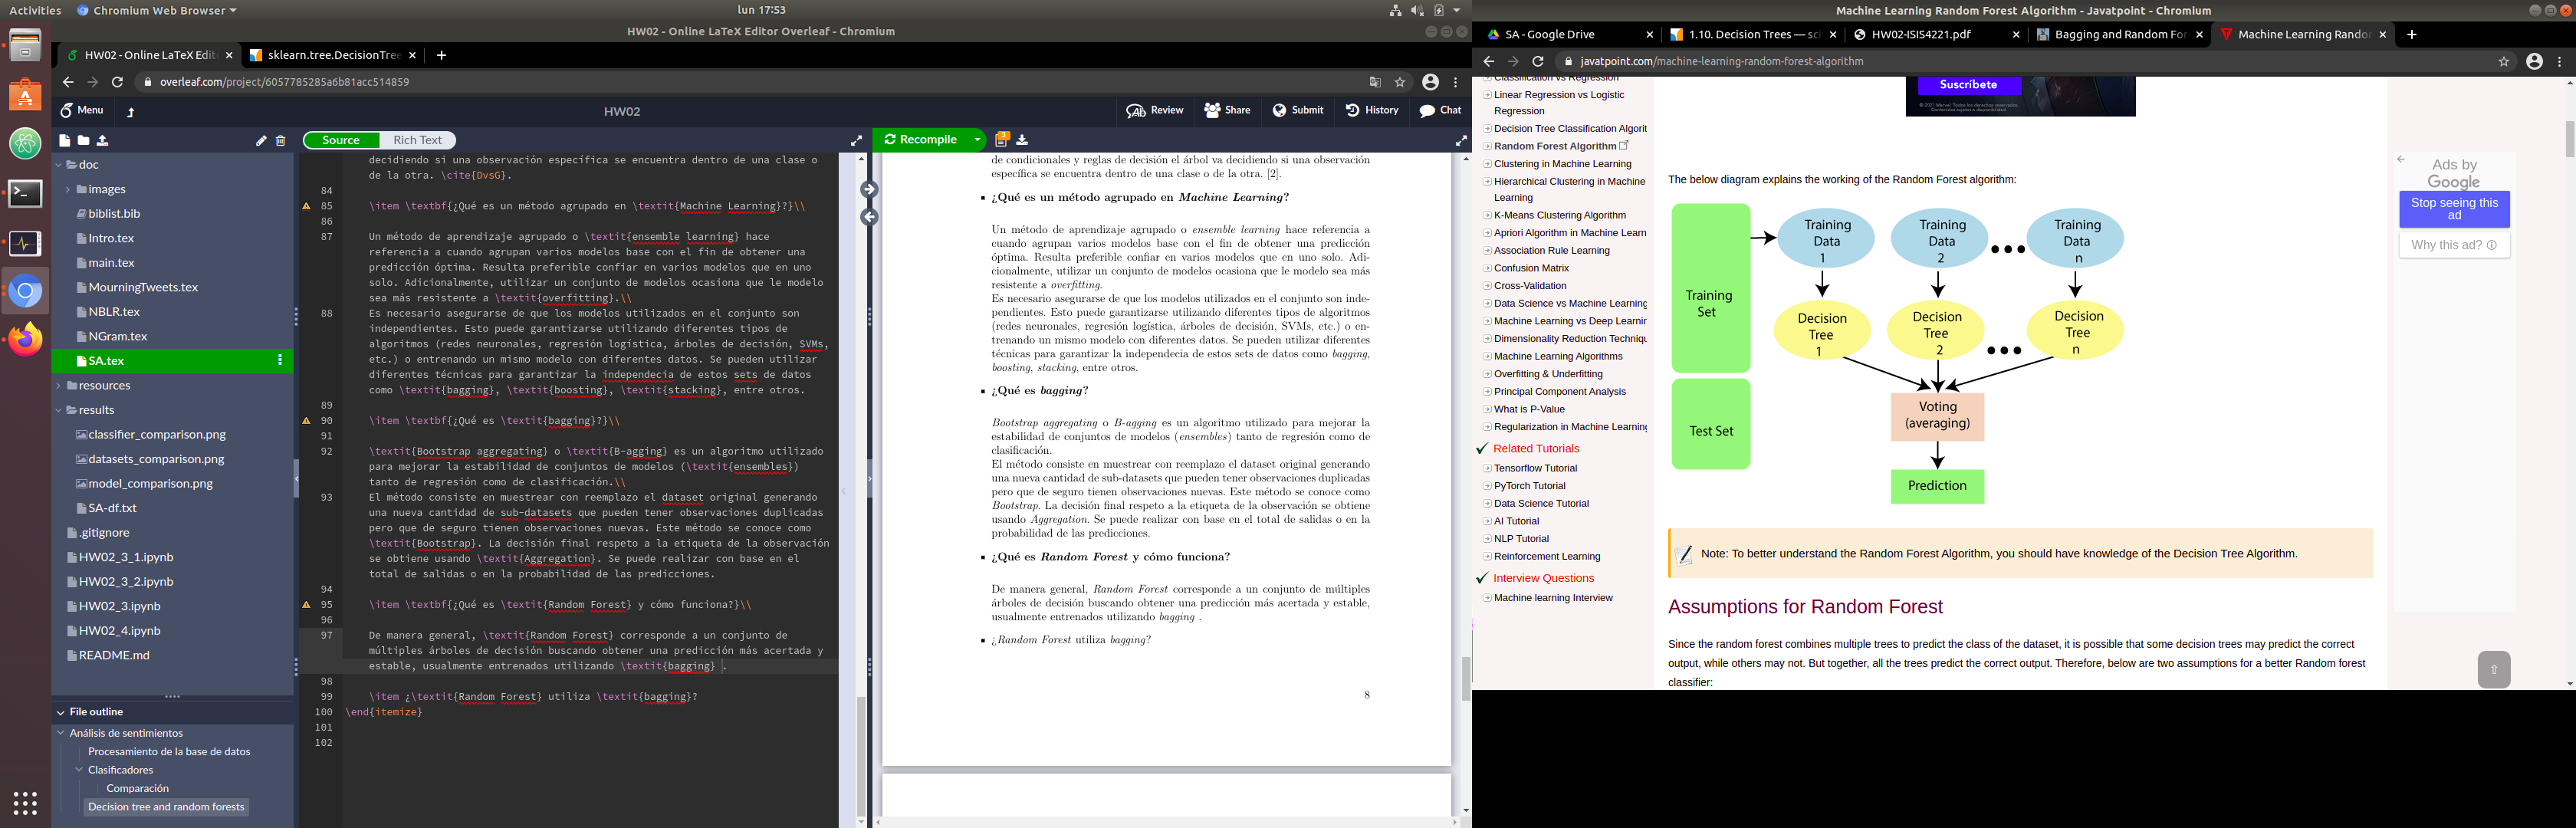
\includegraphics[trim={77cm 15cm 20cm 9cm}, clip, scale = 0.5]{doc/images/randomrofest.png}
        \caption{Random Forest (Tomado de \cite{javatpoint})}
        \label{fig:RF}
    \end{figure}
    
    Cabe resaltar que este algoritmo tiene ventajas en cuanto a que toma menos tiempo de entrenamiento comparado con otros, puede predecir con alto porcentaje de acierto y es capaz de mantener este porcentaje cuando hay una alta porción de datos faltantes \cite{javatpoint}.\\
    El proceso \cite{3} que sigue la creación de un \textit{Random Forest} se muestra a continuación:
    \begin{enumerate}
        \item Seleccionar aleatoriamente K observaciones del set de datos.
        \item Construir K árboles con diferentes set de entrenamiento.
        \item Votación de los K árboles con una observación. Para la votación en algoritmos tareas de clasificación se selecciona \textit{moda} y para regresión se utiliza \textit{media}.
        \item Seleccionar la clase o valor definitivo.
    \end{enumerate}
\end{itemize}

